\documentclass[12pt,a4paper]{article}

\usepackage{geometry}
\usepackage{graphicx}

\geometry{a4paper,top=2.5cm,bottom=2.5cm,left=2.5cm,right=2.5cm}
\usepackage[T1]{fontenc}
\usepackage[utf8]{inputenc}
\usepackage[english]{babel}
\usepackage[parfill]{parskip}

\usepackage{caption}
\captionsetup{font=footnotesize}

%\usepackage{xurl}
\usepackage{hyperref}
\usepackage{graphicx}
\usepackage{booktabs}
\usepackage{tabularx}
\usepackage{wrapfig}
\usepackage{listings}
\usepackage[dvipsnames]{xcolor}
\usepackage{listings}

%Setting listing
\definecolor{mygreen}{rgb}{0,0.6,0}
\definecolor{mygray}{rgb}{0.5,0.5,0.5}
\definecolor{mymauve}{rgb}{0.58,0,0.82}

\lstset{
	basicstyle=\footnotesize\sffamily\color{black},
	frame=single,
	numbers=left,
	numbersep=5pt,
	numberstyle=\tiny\color{gray},
	showspaces=false,
	showstringspaces=false,
	tabsize=1
}

\lstdefinelanguage{Kotlin}{
	comment=[l]{//},
	commentstyle={\color{gray}\ttfamily},
	emph={filter, first, firstOrNull, forEach, lazy, map, mapNotNull, println},
	emphstyle={\color{OrangeRed}},
	identifierstyle=\color{black},
	keywords={!in, !is, abstract, actual, annotation, as, as?, break, by, catch, class, companion, const, constructor, continue, crossinline, data, delegate, do, dynamic, else, enum, expect, external, false, field, file, final, finally, for, fun, get, if, import, in, infix, init, inline, inner, interface, internal, is, lateinit, noinline, null, object, open, operator, out, override, package, param, private, property, protected, public, receiveris, reified, return, return@, sealed, set, setparam, super, suspend, tailrec, this, throw, true, try, typealias, typeof, val, var, vararg, when, where, while},
	keywordstyle={\color{NavyBlue}\bfseries},
	morecomment=[s]{/*}{*/},
	morestring=[b]",
	morestring=[s]{"""*}{*"""},
	ndkeywords={@Deprecated, @JvmField, @JvmName, @JvmOverloads, @JvmStatic, @JvmSynthetic, Array, Byte, Double, Float, Int, Integer, Iterable, Long, Runnable, Short, String, Any, Unit, Nothing},
	ndkeywordstyle={\color{BurntOrange}\bfseries},
	sensitive=true,
	stringstyle={\color{ForestGreen}\ttfamily},
}

%Title
\title{\textbf{QActor Extensions:\\Additional mechanisms to define the model}}
\author{Luca Marchegiani}

\makeindex

\begin{document}
\maketitle

%Body -----------------------------------------------------------------------------------
\section*{Abstract}

In this paper we discuss new mechanisms to define an executable \textit{actor model} using the custom infrastructure and modeling language given by the course of \textit{Ingegneria dei Sistemi Software} of the Bologna university.

The main mechanism that we present is based on \href{https://docs.oracle.com/javase/tutorial/java/annotations/}{\texttt{Java Annotations}}.
\section{Introduction}

\href{http://htmlpreview.github.io/?https://github.com/anatali/issLab2021/blob/main/it.unibo.qakactor/userDocs/LabQakIntro2021.html}{\textbf{\textit{QActor}}} (or \textbf{\textit{QAK}}) is a modeling language to define meta models using \textit{actors}. The language is well explained in the official web page $\big[$ \href{http://htmlpreview.github.io/?https://github.com/anatali/issLab2021/blob/main/it.unibo.qakactor/userDocs/LabQakIntro2021.html}{link} $\big]$.

The \textit{QActor} does not only provide a custom \texttt{DSL}, but also an entire infrastructure that let the developer to design and build basic \textit{actor} systems.
Actually, there are two ways to write systems based on actor modeling using \texttt{QAK}:
\begin{enumerate}
	\item \textit{the custom DSL} made using \href{https://www.eclipse.org/}{\texttt{Eclipse}} and \href{https://www.eclipse.org/Xtext/}{\texttt{Xtext}};
	\item \textit{manually}, writing a description of a system in a \texttt{.pl} file and extending some class of the infrastructure like \href{https://htmlpreview.github.io/?https://github.com/anatali/issLab2021/blob/main/it.unibo.qakactor/userDocs/LabQakIntro2021.html\#ActorBasic}{\texttt{ActorBasic}} or \texttt{ActorBasicFsm}.
\end{enumerate}

Unfortunately, these two mechanisms have some problems:
\begin{enumerate}
	\item the DSL is strongly dependent from \texttt{Eclipse} because it has not an own IDE.
	This can be a problem because the \texttt{QAK} is written in \texttt{Kotlin} and \texttt{Eclipse} is not fully compatible with this language.
	\item writing all things \textit{manually} should be very \textit{uncomfortable}.	
\end{enumerate}

So, in this report we analyze some alternatives to define the actor model according with the \texttt{QAK} infrastructure. We will not go into the details of the \texttt{QActor} implementations because they are fully described into the official web page but we emphasize that the main way to create an actor in this system is:
\begin{center}
	\textbf{Creates a class} that extends \texttt{ActorBasic} or \texttt{ActorBasicFsm} with the body of the actor and \textbf{add a proper description} of it into a file \texttt{.pl}. This file must also contains all the information about the context of the actor and the other actors that can be also remote.\footnote{See the documentation for more details.}
\end{center}

Indeed, the \texttt{DSL} does not do magic: it does nothing more than auto-generate that follows the mechanism the have just described.
As we have already said, we want to extend this in order to have a new mechanism based on \texttt{Java Annotation}.

But before doing this, we also want to find a way to strongly \textbf{separate the actor system description from its runtime implementation}. In fact, if we consider a single actor, actually both of its description and its runtime context are enclosed into the \texttt{ActorBasic} class (or \texttt{ActorBasicFsm}) and its subclass that contains the body.

Then we want to provide a way to define \textit{passive entities} that only contain the description of the actor system you want to define. As these entities will only be used to describe the system, we will call them \textbf{\textit{transient}}. 


\section{The Transient model}
\subsection{Package \texttt{it.unibo.kaktor.model}}

As we have already said, the \textit{transient} model consists in a series of entities that represent the description of the actor system that the application designer want to define.
In a first approximation these entities will then be wrapped into \texttt{ActorBasic} instances that will be used as regular.

We remember that the main entities defined into the \texttt{QA-System} are:
\begin{itemize}
	\item \textbf{actors} active components that are able to receive messages and handle them in a proper way;
	\item \textbf{body} as the main behavior of each actor;
	\item \textbf{messages} as the communication unit for the actors;
	\item \textbf{states} (for finite state machine actors);
	\item \textbf{transitions} (for finite state machine actors);
	\item \textbf{contexts};
\end{itemize}

\begin{figure}[h]
	\centering
	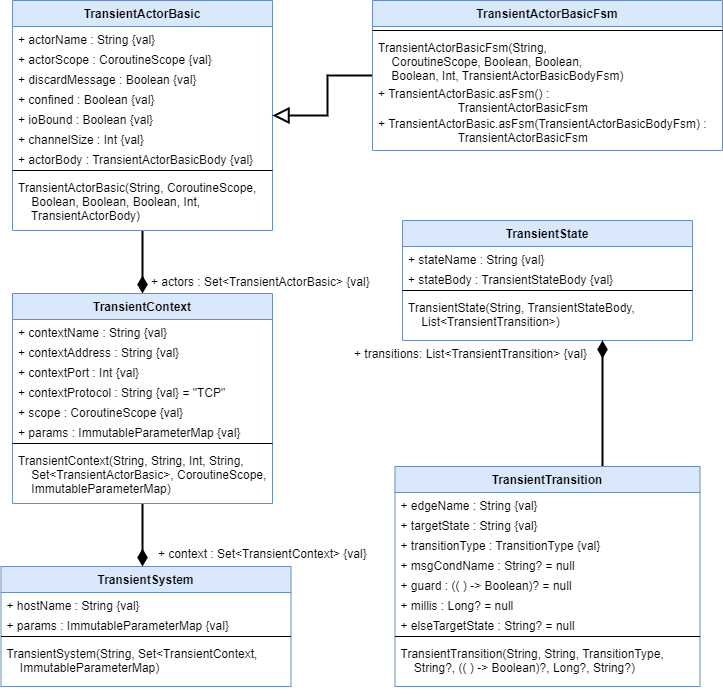
\includegraphics[width=\textwidth]{img/[UML]it.unibo.kaktor.model}
	\caption{UML diagram for the Transient Model}
	\label{fig::uml_model}
\end{figure}

Slightly abusing the \texttt{UML} notation, the figure \ref{fig::uml_model} shows the diagram of the transient model package. We have provided these classes:
\begin{itemize}
	\item
	\underline{\textbf{\texttt{TransientActorBasic}}}:\\
	The class represents the description of an actor (e.g. its name, its scope, its channel size and other options), particularly \textbf{its body} that will be described in a few lines; this is the central class of the model that will be \textit{wrapped} into the \texttt{ActorBasic} class used from the system for the runtime implementation.
	
	\item
	\underline{\textbf{\texttt{TransientActorBasicFsm}}}:\\
	This class represents the description of an actor that is a \textit{finite state machine}. So it extends the \texttt{TransientActorBasic} class but has a \textit{finite state body} instead of the normal body of its super-class.
	
	\item
	\underline{\textbf{\texttt{TransientState}}}:\\
	This class represents the description of a state of a finite state machine actor. It has a 	\textit{name} and a \textit{state body} that will be called when a \textit{FSM} actor enters the state.
	
	\item
	\underline{\textbf{\texttt{TransientTransition}}}:\\
	This class represents the description of a transition from one state to another into a \textit{FSM} actor. So it has an \textit{edge name} used to identify uniquely the transition, a \textit{target state} and a \textit{type}. Based on the type it also has additional fields used be the specific type.
	
	\item 
	\underline{\textbf{\texttt{TransientContext}}}:\\
	This class represents the description of a context that contains a collection of actors. In addition to this, a context also have some field that describes some of its characteristics (like its name, its address and so on).
	
	\item 
	\underline{\textbf{\texttt{TransientSystem}}}:\\
	This class represents the description of the entire system that will be executed. As a \texttt{TransientContext} it also has a \texttt{ImmutableParameterMap} that is an object defined in another package that maintains a series of key-object pairs for re-usability.
	\textbf{This is the end class of the \textit{transient model} that will be passed to method that load and build the entire system}.
\end{itemize}

\subsection{Package \texttt{it.unibo.kaktor.model.actorbody}}

We have shown that the \texttt{TransientActorBasic} class maintains an object that represents the actor body. Same for the \texttt{TransientActorBasicFsm} class in which the difference is that the body has the behavior of a finite state machine.

\begin{figure}[h]
	\centering
	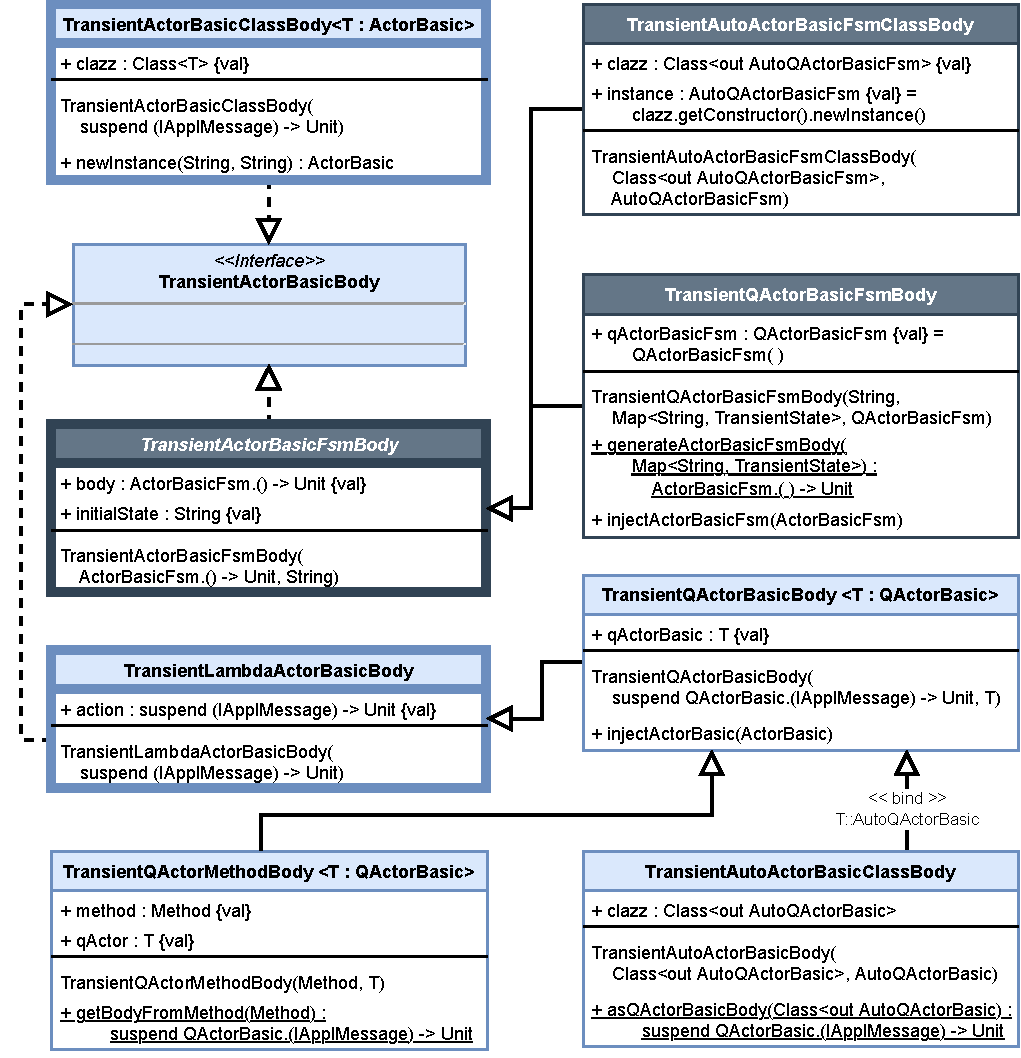
\includegraphics[width=\textwidth]{img/[UML]it.unibo.kaktor.model.actorbody_onlyactorbody}
	\caption{UML diagram for the Transient Model of the actor body}
	\label{fig::uml_model_body}
\end{figure}

The figure \ref{fig::uml_model_body} summarizes the package that contains the class for the actor body. The main classes of this package are:

\begin{itemize}
	\item 	\underline{\textbf{\texttt{TransientActorBasicBody}}}:\\
	This classes that implements this symbolic interface are actor basic bodies.
	
	\item 	\underline{\textbf{\texttt{TransientLambdaActorBasicBody}}}:\\
	This is the main class for a body of an \texttt{ActorBasic} instance. It maintains a \href{https://kotlinlang.org/docs/lambdas.html}{\textit{lambda function}} that describes the actions the actor will have to perform when receives a message.
	
	\item 	\underline{\textbf{\texttt{TransientActorBasicFsmBody}}}:\\
	This is the main class for a body of an \texttt{ActorBasicFsm} instance. It maintains a \href{https://kotlinlang.org/docs/lambdas.html#closures}{\textit{lambda function with closure}} that contains the actions to be create an instance of the \texttt{ActorBasicFsm} class\footnote{See the official \texttt{QAK} documentations for details about the creation of a finite state machine actor.} and also the name of the initial state.
\end{itemize}

The other classes of this package are useful in order to easily create instances of these main superclasses and will be clarified soon.

\begin{figure}[h]
	\centering
	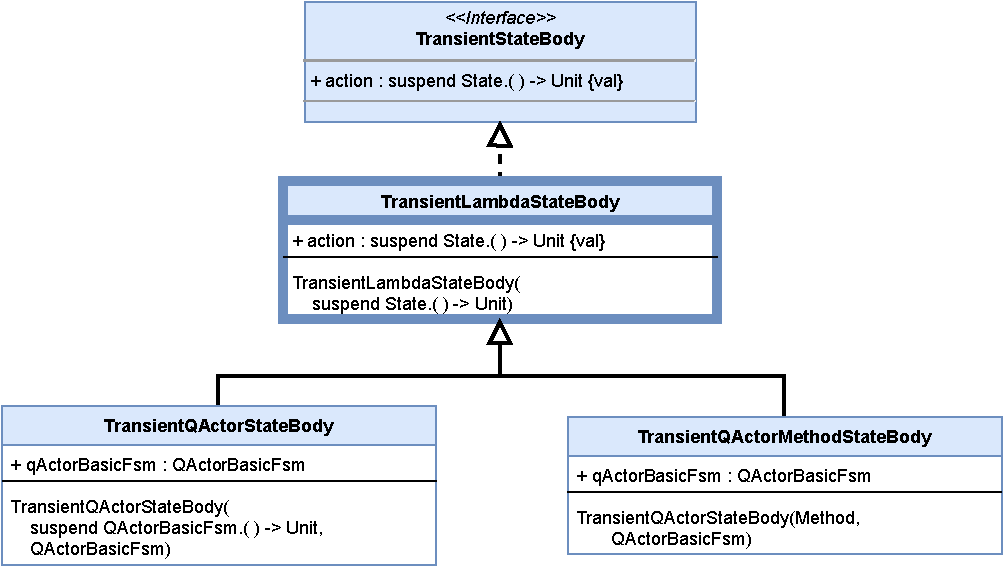
\includegraphics[width=\textwidth]{img/[UML]it.unibo.kaktor.model.actorbody_onlystatebody}
	\caption{UML diagram for the Transient Model of the actor body}
	\label{fig::uml_model_state_body}
\end{figure}

The figure \ref{fig::uml_model_state_body} shows the classes describing the body of a state. It contains:
\begin{itemize}
	\item 	\underline{\textbf{\texttt{TransientStateBody}}}:\\
	This classes that implements this symbolic interface are finite state machines bodies.
	
	\item 	\underline{\textbf{\texttt{TransientLambdaStateBody}}}:\\
	This is the main class for a body of a finite state machine. It maintains a \href{https://kotlinlang.org/docs/lambdas.html}{\textit{lambda function}} that describes the actions the actor will have to perform when enters the state owning this body.
\end{itemize}
The other two subclasses will be used to easily create instance of lambda state body and will be explained in the next sections.





\section{The builder mechanism}

\subsection{Overview of the builder package \texttt{it.unibo.kaktor.builders}}

In addition to the transient model, we want to provide a sort of \textit{standard mechanism} that must be reliable and reusable to create the transient entities.

So, we decided to use the \href{https://en.wikipedia.org/wiki/Builder_pattern}{builder pattern}.

\begin{figure}[h!]
	\centering
	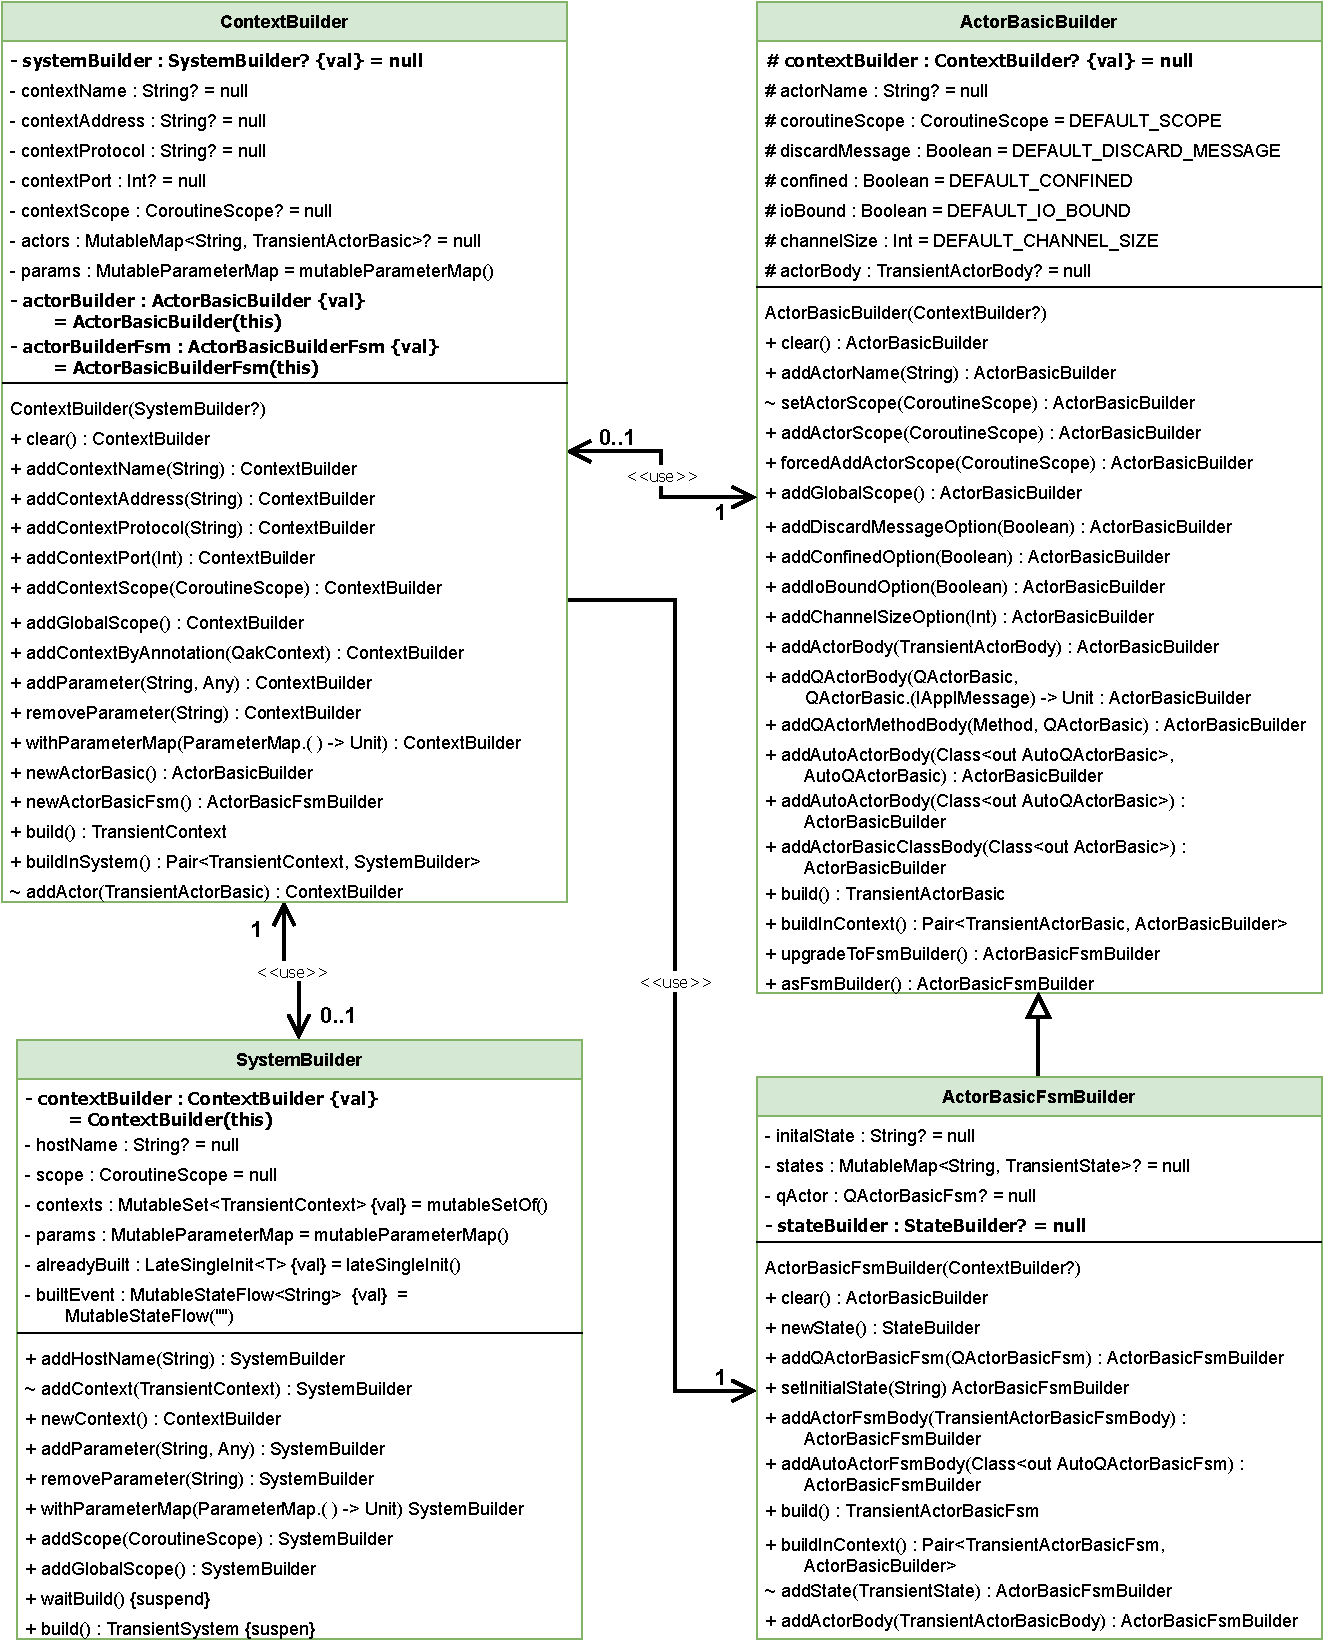
\includegraphics[width=0.92\textwidth]{img/[UML]it.unibo.kaktor.builders_actorb_contextb_systemb}
	\caption{UML diagram for the actor, context and system builders}
	\label{fig::builders_actorb_contextb_systemb}
\end{figure}

The figure \ref{fig::builders_actorb_contextb_systemb} shows the main builder components for the transient system. They are:
\begin{itemize}
	\item 	\href{https://github.com/LM-96/QA-Extensions/blob/main/it.unibo.qakactor/src/main/kotlin/builders/ActorBasicBuilder.kt}{\underline{\textbf{\texttt{ActorBasicBuilder}}}}:\\
	This component let to create a \texttt{TransientActorBasic} using the builder pattern. It is easy possible to set the actor body by calling the \verb*|addActorBoby(TransientActorBody)| method. There are others additional methods that can be used to quickly add  more complex body that the normal lambda body (the classes not already explained of the transient body model).
	
	\item 	\href{https://github.com/LM-96/QA-Extensions/blob/main/it.unibo.qakactor/src/main/kotlin/builders/ActorBasicFsmBuilder.kt}{\underline{\textbf{\texttt{ActorBasiFsmcBuilder}}}}:\\
	This component let to create a \texttt{TransientActorBasicFsm} using the builder pattern. This class extends the \texttt{ActorBasicBuilder} then add others additional method to its in order to create a finite state machine actor. It is easy possible to add a state to the actor that is building by calling \verb*|newState()| method that returns a \texttt{StateBuilder} for the new state.
	
	\item 	\href{https://github.com/LM-96/QA-Extensions/blob/main/it.unibo.qakactor/src/main/kotlin/builders/ContextBuilder.kt}{\underline{\textbf{\texttt{ContextBuilder}}}}:\\
	This component let to create a \texttt{TransientContext}. It is easy possible to add an actor to the context that is building by calling \verb*|newActorBasic()| or \verb*|newActorBasicFsm()| methods that return a builder for the new actor.
	
	\item 	\href{https://github.com/LM-96/QA-Extensions/blob/main/it.unibo.qakactor/src/main/kotlin/builders/SystemBuilder.kt}{\underline{\textbf{\texttt{SystemBuilder}}}}:\\
	This component let to create a \texttt{TransientSystem}. It is easy possible to add a context to the system that is building by calling \verb*|newContext()| method that returns a \texttt{ContextBuilder}. When the creation of the transient system is completed so it is needed to invoke the \verb*|buil()| method that returns the \texttt{TransientSystem}. Notice that \textbf{a \texttt{SystemBuilder} cannot be reused then once the system is created it not possible to clear the builder and start again the creation}. In addition to this, after the build method invocation, there are no possibilities to add other contexts or to build again.
\end{itemize}

In addition to all things we have just explained, the builders can throw a \texttt{BuildException} if something goes wrong or if the developer has not passed all the needed information to it before invoking \verb*|build()|, for example if the developer invoke it without calling the \verb*|addActorName(String)| before.

\begin{figure}[h!]
	\centering
	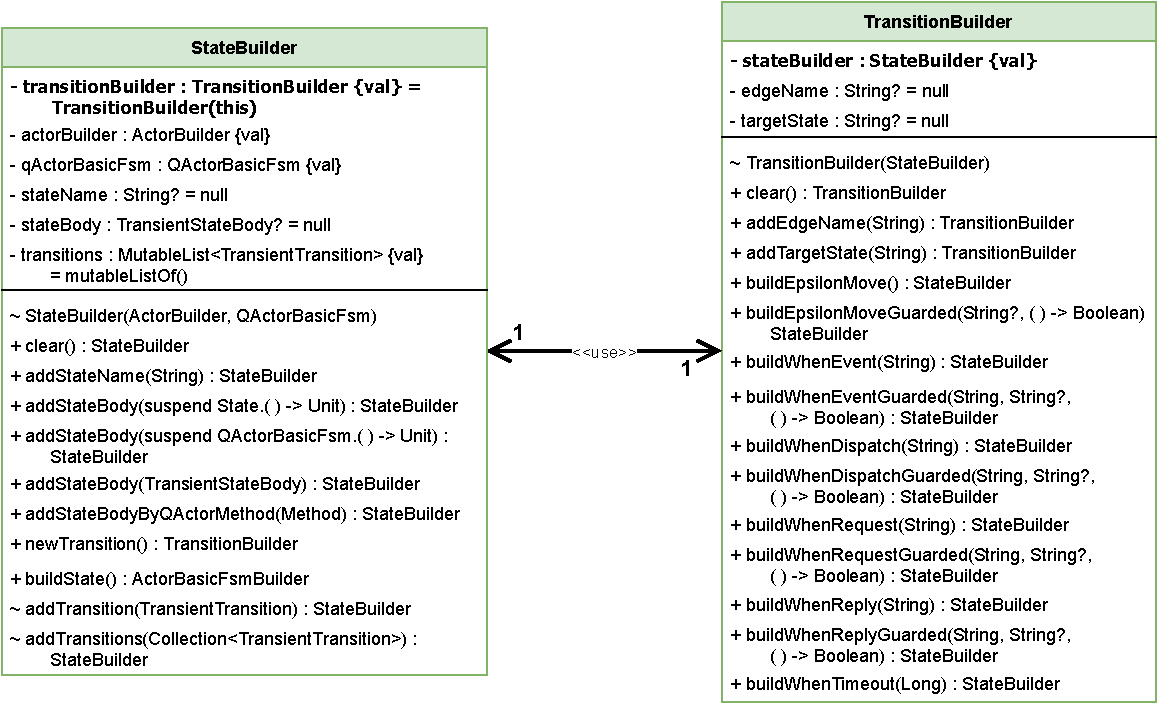
\includegraphics[width=\textwidth]{img/[UML]it.unibo.kaktor.builders_stateb_transitionb}
	\caption{UML diagram for the for the state and transition builders}
	\label{fig::builders_stateb_transitionb}
\end{figure}
As anticipated, for finite state machine actors we also provide some additional builders shown in the figure \ref{fig::builders_stateb_transitionb}:

\begin{itemize}
	\item 	\href{https://github.com/LM-96/QA-Extensions/blob/main/it.unibo.qakactor/src/main/kotlin/builders/StateBuilder.kt}{\underline{\textbf{\texttt{StateBuilder}}}}:\\
	The component for building states. If we have an \texttt{ActorBasicFsmBuilder} we can call the \verb*|newState()| method that returns an instance of the \texttt{StateBuilder} class that can be used to add states. When all of the states are added then it is possible to invoke the \texttt{buildState()} method that return the original actor builder. \textbf{Notice that it not possible to create a \texttt{StateBuilder} because it can only be obtained from an actor builder}.
	
	\item 	\href{https://github.com/LM-96/QA-Extensions/blob/main/it.unibo.qakactor/src/main/kotlin/builders/TransitionBuilder.kt}{\underline{\textbf{\texttt{TransitionBuilder}}}}:\\
	The component for building transitions. It can be obtained using the \verb*|newTransition()| method of the \texttt{StateBuilder} class with the same mechanism by which the state builder can be obtained from the actor builder. In addition, this component has more than one \texttt{build} method for each type of transition supported by the infrastructure.
\end{itemize}

\subsection{The wrappers}

As we have already said, the transient entities of the model are only a \textbf{passive description} of the system that will have to run. So this description must be transformed into the \textbf{executable units} that are present in the \texttt{QA} infrastructure: \texttt{ActorBasic} and \texttt{ActorBasicFsm}.

\begin{figure}[h!]
	\centering
	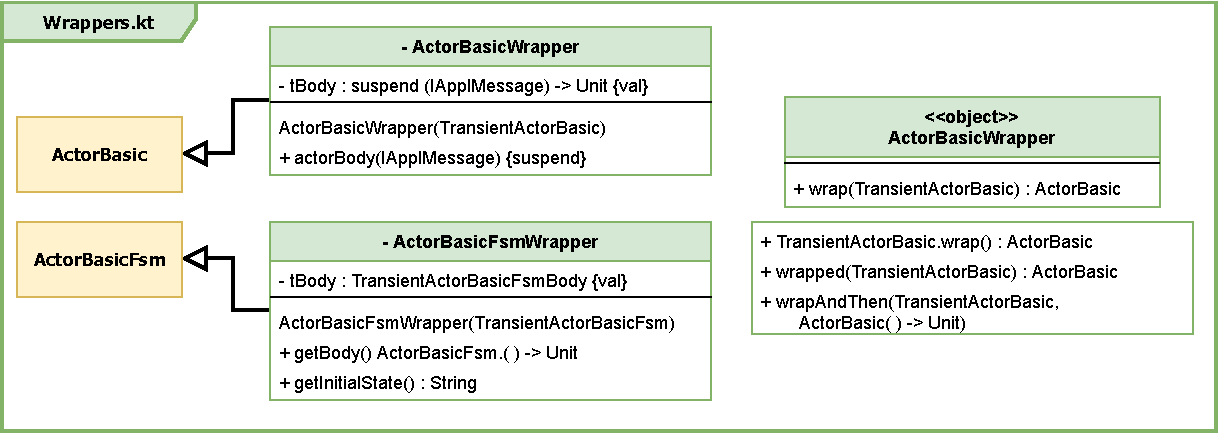
\includegraphics[width=\textwidth]{img/[UML]it.unibo.kaktor.builders_wrapper}
	\caption{UML diagram for the wrappers}
	\label{fig::builders_wrapper}
\end{figure}

The \href{https://github.com/LM-96/QA-Extensions/blob/main/it.unibo.qakactor/src/main/kotlin/builders/Wrappers.kt}{\texttt{Wrappers.kt}} file contains the classes to \textbf{wrap} the \texttt{TransientActorBasic} and the \texttt{TransientActorBasicFsm} entities into the active entities of the \texttt{QA-System}.
This file also contains some extensions method for the \texttt{TransientActorBasic} class to quickly wrap it into an \texttt{ActorBasic} instance.

For the details about wrappers and their work, please see \href{https://github.com/LM-96/QA-Extensions/blob/main/it.unibo.qakactor/src/main/kotlin/builders/Wrappers.kt}{the source code}.

\subsection{Example of system creation using builders}

Suppose to have a system with a context that contains an actor called \textit{echoactor} with this behavior:
\begin{figure}[h!]
	\centering
	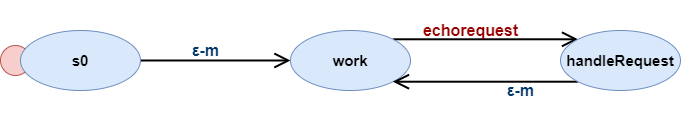
\includegraphics[width=\textwidth]{img/[EG]simple_echo_actor_diagram}
	\caption{Behavior of the \textit{echoactor}}
	\label{fig::echo_actor_example}
\end{figure}

This simple actor is able to handle a request called \texttt{echorequest} by answering with an \texttt{echoresponse} reply containing the same contents of the request.
Then, in order to define the system using the builders, the procedure is:


\begin{lstlisting}[caption={Example of builders use},label={lst::echoexample},language=kotlin]
/* BODIES OF THE STATES FOR echoactor ***************************** */
val s0Body : suspend QActorBasicFsm.()-> Unit =
	{ println("started") }
val workBody : suspend QActorBasicFsm.() -> Unit =
	{ println("idle") }
val handleRequestBody : suspend QActorBasicFsm.() -> Unit =
	{ answer("echorequest", "echoreply", currentMsg.msgContent()) }

/* SYSTEM BUILDER ************************************************* */
val sysBuilder = SystemBuilder()

/* SYSTEM CREATION ************************************************ */
val system = runBlocking {
	sysBuilder.addHostname("localhost").addScope(this)
	//Context: "ctxecho"
	.newContext()
	.addContextName("ctxecho")
	.addContextAddress("localhost").addContextPort(9000)
	.addContextProtocol("TCP")
	//Actor: "echoactor"
	.newActorBasic().addActorName("echoactor")
	.upgrateToFsmBuilder().addQActorBasicFsm(QActorBasicFsm())
				//State: "s0"
	.newState().addStateName("s0").addStateBody(s0Body)
	.newTransition()
	.addEdgeName("t0").addTargetState("work")
	.buildEpsilonMove().buildState()
	.setInitialState("s0")
				//State: "work"
	.newState().addStateName("work").addStateBody(workBody)
	.newTransition()
	.addEdgeName("t1").addTargetState("handleRequest")
	.buildWhenRequest("echorequest").buildState()
				//State: "handleRequest
	.newState().addStateName("handleRequest")
	.addStateBody(handleRequestBody)
	.newTransition()
	.addEdgeName("t2").addTargetState("work").buildEpsilonMove()
	.buildState()
	.buildInContext().second.buildInSystem().second.build()
}
\end{lstlisting}

The \texttt{.kt} source code is available \href{https://github.com/LM-96/QA-Extensions/blob/main/it.unibo.qakactor/src/main/kotlin/demo/EchoExample.kt}{here}.

At the end of the execution of this snippet, the \verb*|system| variable contains the \texttt{OOP} description of the actor system with the \texttt{echoactor} described in the figure \ref{fig::echo_actor_example}.

The motivations for the line $22$ (\verb*|addQActorBasicFsm(QActorBasicFsm())|) will be clarified in the next section.

\subsection{The last step for builders: adding support for make \texttt{TransientSystem} runnable}

In the previous example we have created a complete description of the system contained into the \verb*|system| variable. But what do we do with this now? How we can run the \texttt{TransientSystem}?

In order to do it, \textbf{we have to modify the launching methods of the \texttt{QA-System}}.
Without going into details, we have created a new method into the \href{https://github.com/LM-96/QA-Extensions/blob/main/it.unibo.qakactor/src/main/kotlin/QakContext.kt}{QakContext.kt} that has this signature:

\begin{center}
	\begin{tabular}{c}
		\begin{lstlisting}[frame=none,numbers=none,language=Kotlin]
			fun createSystem(transientSystem : TransientSystem)
		\end{lstlisting}
	\end{tabular}
\end{center}

This method \textcolor{BrickRed}{\textbf{creates and run the system}} starting from a \texttt{TransientSystem} instance.
In addition to this, we have created lots of method into the \href{https://github.com/LM-96/QA-Extensions/blob/main/it.unibo.qakactor/src/main/kotlin/sysUtil.kt}{\texttt{sysUtil.kt}} utility that helps the \verb|createSystem()| to do its work such as:
\begin{center}
	\begin{tabular}{c}
		\begin{lstlisting}[frame=none,numbers=none,language=Kotlin]
			fun createSystem(tSystem: TransientSystem, start : Boolean = true)
			fun createContext(tCtx : TransientContext, hostName: String) : QakContext?
			fun addTheActors(ctx: TransientContext, qakCtx : QakContext )
		\end{lstlisting}
	\end{tabular}
\end{center}
which follows the methods that were used by the old mechanism.

In order to conclude the example of the \ref{lst::echoexample}, we must add this line to run the system:
\begin{lstlisting}[language=Kotlin]
	QakContext.createSystem(system)
\end{lstlisting}



%----------------------------------------------------------------------------------------

\end{document}